% ------------------------------------------------------------------------
% ------------------------------------------------------------------------
% ------------------------------------------------------------------------
%                                Anexo B
% ------------------------------------------------------------------------
% ------------------------------------------------------------------------
% ------------------------------------------------------------------------
% ------------------------------------------------------------------------
\newpage
\anexo{Funci�n \emph{ode45} de MATLAB}\label{anexoB}
% ------------------------------------------------------------------------
\noindent La funci�n $ode45$ est� basada en un algoritmo de tipo Runge-Kutta, que se desarroll� a partir del m�todo de Euler mejorado \citep{chapra2003metodos}. La funci�n recibe tres par�metros esenciales: $f(t)$ dentro de un $script$ en el que se define la ecuaci�n diferencial acompa�ado por un simbolo $@$, el vector de l�mites de tiempo $\left[ t_0 \quad t_f \right]$ y el vector de condiciones iniciales $y_0$. En otras palabras el prototipo b�sico para usar \emph{ode45} es el siguiente:
% ------------------------------------------------------------------------
\begin{equation}\label{defode}
   [t,y]=\emph{ode45}(@f(t),\left[ t_0 \quad t_f \right],y_0);
    \end{equation}
% ------------------------------------------------------------------------
En este caso la soluci�n num�rica se almacenar� en el vector $y$  para cada uno de los instantes de tiempo presentes en el vector $t$.\\

La funci�n $ode45$, resuelve ecuaciones del tipo $\dot{y} = f(t,y)$, por tanto si se desea resolver ecuaciones de orden superior estas deben escribirse como un sistema de ecuaciones diferenciales de primer orden.\\

A manera de ejemplo, se ilustrar� la forma de resolver la ecuaci�n diferencial de segundo orden
% ------------------------------------------------------------------------
\begin{equation}\label{segundo}
   \ddot{x}-\mu\left(1-x^2\right)\dot{x}+x=0,
\end{equation}
% ------------------------------------------------------------------------
donde $\mu > 0$ es un par�metro escalar.\\

Por tanto, definiendo
% ------------------------------------------------------------------------
$$y_1 = x; \quad y_2 = \dot{x}$$
% ------------------------------------------------------------------------
la expresi�n \eqref{segundo} puede ser reescrita como
% ------------------------------------------------------------------------
$$
\dot{y}_2 = \mu \left( 1 - y_1^2 \right) y_2 + y_1
$$
% ------------------------------------------------------------------------
es decir, transformando la ecuaci�n diferencial original de segundo orden y una variable, en una ecuaci�n diferencial equivalente de primer orden y dos variables. As� entonces, es posible construir el vector
% ------------------------------------------------------------------------
$$
y = \left[ {\begin{array}{*{20}c}
   y_1  \\
   y_2  \\
\end{array}} \right]
$$
% ------------------------------------------------------------------------
cuya din�mica viene representada por
% ------------------------------------------------------------------------
$$
\dot{y} = \left[ {\begin{array}{*{20}c}
   f_1 \left(t, y \right)  \\
   f_2 \left(t, y \right) \\
\end{array}} \right]
$$
% ------------------------------------------------------------------------
siendo
% ------------------------------------------------------------------------
$$f_1\left(t, y \right) = y_2; \quad f_2\left(t, y \right) =  \mu \left( 1 - y_1^2 \right) y_2 + y_1$$
% ------------------------------------------------------------------------
De esta manera, evaluar la expresi�n \eqref{defode} permite obtener una matriz de salida $y$ con filas representando los vectores soluci�n para $y_1$ e $y_2$ como funci�n de $t$.\\
% ------------------------------------------------------------------------

\begin{figure}[h]
\centering
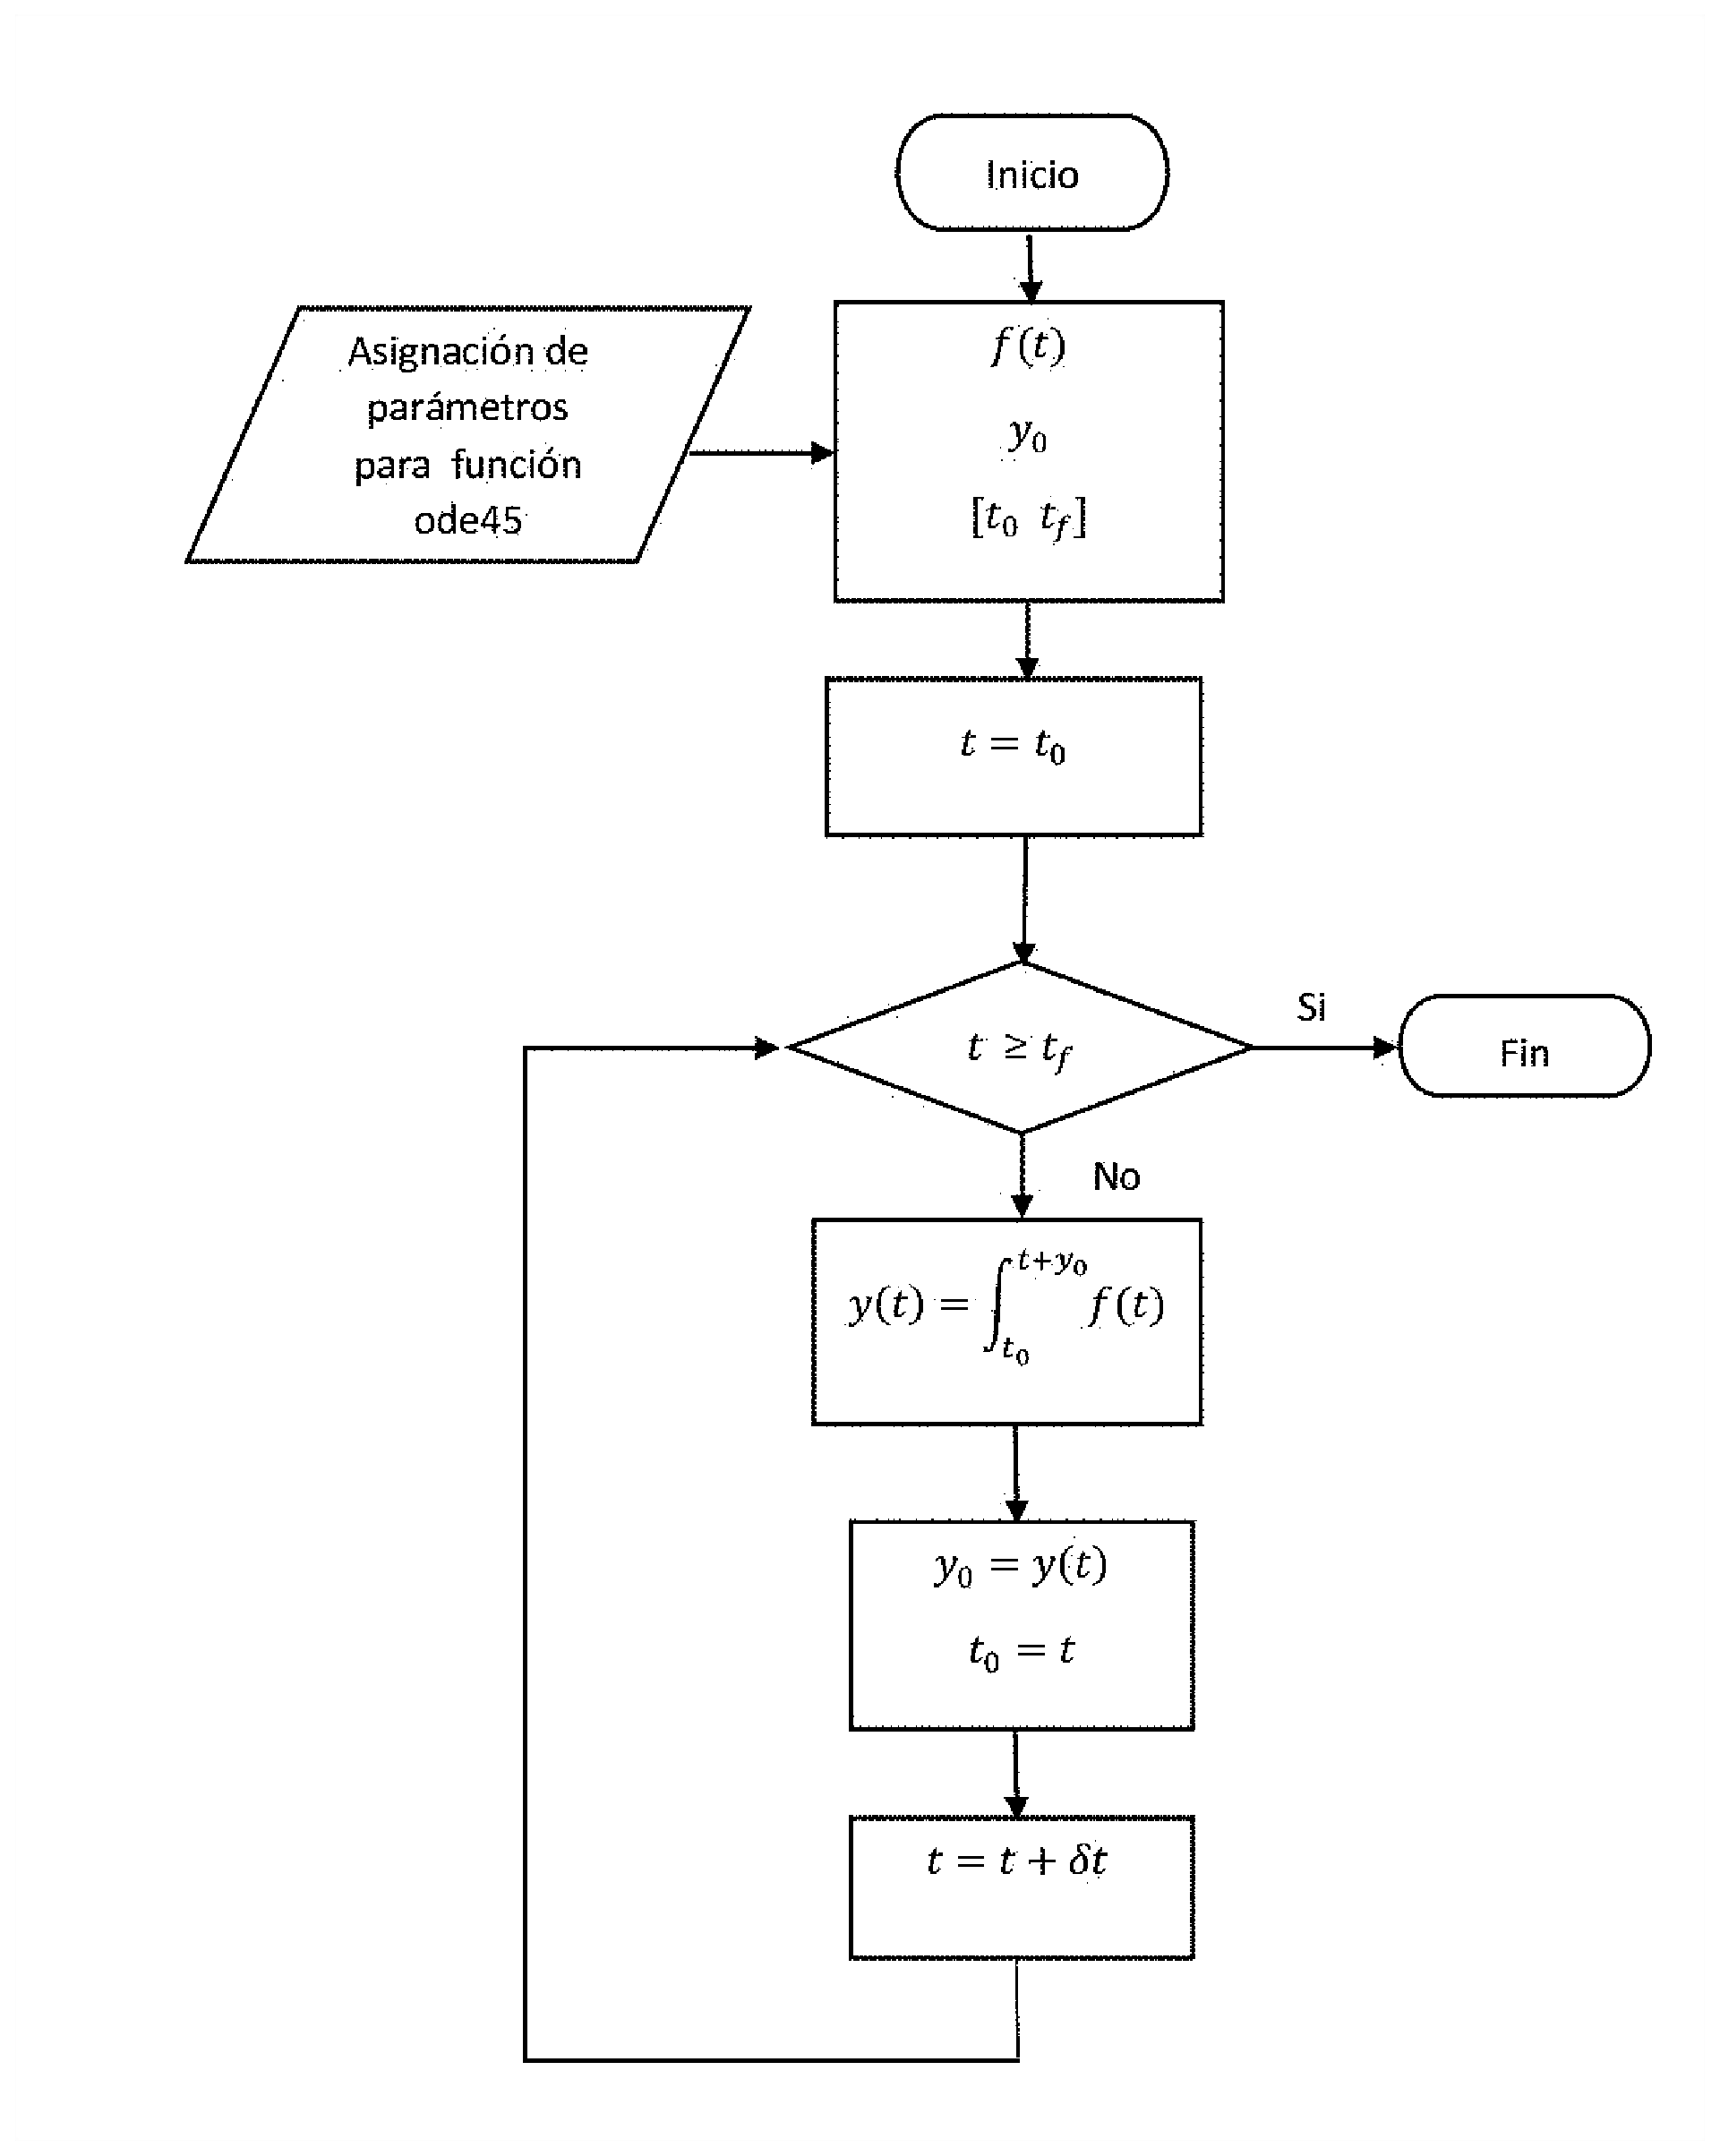
\includegraphics[width=0.55\textwidth]{Figs/flujodiag}
\caption[]{Diagrama de flujo para algoritmo de integraci�n num�rica de la funci�n $ode45$ de MATLAB}\label{flujodiag}
\end{figure}
% ------------------------------------------------------------------------

En la Fig. \ref {flujodiag} se ilustra el diagrama de flujo del algoritmo empleado para hallar la soluci�n de una ecuaci�n diferencial mediante integraci�n num�rica empleando la funci�n $ode45$ de MATLAB.\\

Inicialmente, se deben asignar los par�metros definidos en la ecuaci�n \eqref{defode}.\\

Posteriormente, un bucle interno hace llamado iterativo a la funci�n $f(t)$ evaluada para valores de tiempo entre $t_0$ y $t_f$ a partir de las condiciones iniciales $y_0$. Para cada ciclo la condici�n inicial se recalcula siendo la condici�n final del ciclo anterior. El tiempo se incrementa en un tama�o de paso $\delta t$ de forma adaptativa, si no se especifica lo contrario. Tras alcanzarse el tiempo final $t_f$, el bucle interno termina y entrega como resultado el vector de puntos de la trayectoria soluci�n $y(t)$ al igual que el vector de tiempos $t$. 